\section{Results}
\subsection{Adaptation}\label{adapt_section}
	A population of random 400-node seed networks, each having an edge:node ratio matching that of the Yeast network (Table \ref{networks_summary})\footnote{The real BNs used in this study (Table \ref{networks_summary}) are publicly available in: \url{http://cs.mcgill.ca/~malsha17/permlink/acmbcb17/}}, 
	is subjected to successive rounds  of RVnRS. 
	The evolutionary algorithm mutates each network in the population by edge-reassignment only and subsequently 
	selects the fittest networks (according to their $F(S)$ values) to breed the next population of networks.
	The networks are sorted according to fitness, and the top 10\% are selected. 
	Replicas are produced from each selected network bringing the population to its previous size. Figure \ref{adap_fig} (a) displays 
	the degree distribution of the fittest adapted network after 2000  mutate-select-breed generations (black dots) against 
	100 400-node randomly sampled subnetworks from Yeast. 
	The connectivity of of the adapted network morphed into the mLmH property matching that of Yeast. 
	Figure \ref{adap_fig} (b) shows the change in the overall 
	fitness score of the fittest network in the population at each generation (top) as well as the change in fitness score per metric 
	($U^2$ (left) and $\frac {B_e}{B_{tot}}$ (right) subplots). The fitness improves dramatically at the beginning and plateaus by generation 2000. 
	The remaining fluctuations are largely due to variance in NEP as different instances may vary in fitness for the same network. 
	$U$ and $\frac {B_e}{B_{tot}}$ are balance the two competing forces of selecting for unambiguity (leaf nodes) and effective total benefits (hub nodes). 

	Figure \ref{adap_fig} (c) depicts the percent of unambiguous nodes at the beginning and end of the simulation. The adapted network at generation 2000 
	has more leaf nodes contributing to the unambiguous 100:0 and 0:100 $benefit$:$damage$ ratio groups. The random network exhibits 35.9\% unambiguous nodes (solid red and green slices), whereas 
	the evolved network results in 53.5\% unambiguous nodes. The latter clearly produces NEP instances with small effective instance sizes. 
	Figure \ref{adap_fig}(d) portrays the composition of the NEP solution. Adapted networks fit larger hubs into the solution due to 
	the fact that the more leaf nodes a network has the less threshold damage is consumed and therefore hubs (which are likely to 
	carry damaging interactions) are more likely to  be conserved (i.e. part of the optimal solution) for their benefits and despite their damages. 
	That implies that a hub involved in damaging interactions 
	can still be tolerated while more experimentation in network composition (conserve/delete) and/or connectivity (mutations that 
	affect interaction affinity) can take place \cite{kim_positive_2007}. 
	Figure \ref{adap_fig} (e)  
	displays the change in degree distribution on a normal and a log-scaled (inset) plot. The seed networks at 
	the first generation are created by randomly assigning edges resulting in an 
	exponential degree distribution centred around the average degree. In stark contrast, adapted networks at generation 2000
	display a heavy-tailed distribution with a few highly
	connected hubs. The model robustly evolves to mLmH topology despite unfavourable starting conditions. Very low degree (leaf) nodes dramatically increase in 
	frequency, while more high-degree (hub) nodes emerge. 
%
\subsection{Adaptation with Growth}\label{evolution_results}
	The same evolutionary algorithm is applied starting from a near empty seed network that grows in size
	over the generations. Networks in the population start with 4 nodes and periodically acquire new nodes 
	and edges. Figure \ref{evol_figure} illustrates simulated networks and their corresponding
	BNs that have the same edge:node ratio. The BNs are protein-protein interaction networks of 6 different organisms. The simulation is terminated when the simulation network
	reaches the size of 400 nodes. For comparison, 
	 100 400-node subnetworks are sampled from the corresponding BN (colour dots in Figure \ref{evol_figure}). 
	 The degree distributions of simulated networks (black dots in Figure \ref{evol_figure})
	closely match their corresponding BNs. 
	%The simulation also replicates the tendency  for BNs to increase leaves at lower edge to node ratios. 
	%Sampled subnetworks from BNs may include larger hubs, since larger networks have more edges to produce highly connected nodes. 
	The frequency of hubs in  networks sampled from real BNs is comparable to those resulting from simulations, although the latter have lower probability of generating
	extremely highly connected hubs given their smaller size.  
\begin{comment}
Fitness is based on a leaf metric that emphasizes sparsely connected nodes and a hub metric that promotes highly connected nodes. Fitness is the product of these two forces, which stretch the degree distribution in both directions to exhibit heavy-tailed connectivity. 

$f(N)=LF \times HF$

The leaf metric is based on minimizing the correlation between benefits and damages. Previous work demonstrates that higher correlation between values and weights result in more computationally expensive knapsack problems \cite{pisinger_where_2005}. Nodes are evaluated based on the ratio of benefits to all interactions (benefits + damages). The symmetrical case of damages to all interactions is also considered, and the higher outcome is preferred. Lower degree nodes are far more likely to be uncorrelated. The ratio alone vastly prefers degree one, so the square root of the ratio is taken to create smoother spectrum. The total leaf fitness is the average of the fitness of all nodes. 

$LF = \frac { |\{g_i: b_i = 0 | d_i=0\}| }  {|G|}$

The hub metric captures the ability to garner more benefits with less change. The benefits of the nodes in solution to the NEP is transformed from a multi set to a single set, which removes redundant numbers. The hub metric is composed of the sum of the single set of the benefits in the solution, divided by the sum of the multi set of benefits in the solution. Since the solution tends to include many small elements, the metric evaluates the proportion of the solution that is due to large, infrequent elements.

$HF = \frac { |\{g_i: b_i = 0 | d_i=0\}| }  {\sum\limits_{i=1}^{n} b_i}$
\end{comment}
\setlength{\textfloatsep}{0pt plus 1.0pt minus 1.0pt} % http://tex.stackexchange.com/questions/26521/how-to-change-the-spacing-between-figures-tables-and-text
	\begin{table}[t] %h:here, t:top of page, b:bottom of page, more: http://tex.stackexchange.com/questions/35125/how-to-use-the-placement-options-t-h-with-figures
		%\setlength\arrayrulewidth{.1pt}\arrayrulecolor[HTML]{0a84f7} %https://en.wikibooks.org/wiki/LaTeX/Colors#Adding_the_color_package
		\scriptsize %\small \tiny, \scriptsize, \footnotesize, \small, \normalsize, \large, \Large, \LARGE, \huge, and \Huge.
			\setlength\cellspacetoplimit{4pt} % padding in table cells
			\setlength\cellspacebottomlimit{4pt} %padding in table cells
			\begin{tabular}{c|c|c|c}  % http://tex.stackexchange.com/questions/302960/modify-arraystretch-for-a-single-row-in-table
				\hline\hline
					\textbf{Network} & \textbf{no. nodes} & \textbf{no. edges}	& \textbf{edge:node ratio}
				\\[.05cm] \hline
					Plant \cite{consortium_evidence_2011}  & 2402 & 5486 & 2.3
				\\[.05cm] \hline
					Bacteria \cite{rajagopala_binary_2014} & 1014 & 1967 & 1.9
				\\[.05cm] \hline
					Yeast \cite{yu_high-quality_2008}      & 1647 & 2682 & 1.6
				\\[.05cm] \hline
					Worm \cite{simonis_empirically_2009}   & 2214 & 3659 & 1.7
				\\[.05cm] \hline
					Fly \cite{vinayagam_integrating_2014}  & 3058 & 5930 & 1.9
				\\[.05cm] \hline
					Human \cite{yang_widespread_2016}      & 473  & 885 & 1.9
				\\[.05cm] \hline
				    Bacteria Regulatory \cite{gama-castro_regulondb_2016} & 898 & 1481 & 1.6
				\\[.05cm] \hline
				    Mouse Regulatory \cite{liu_regnetwork:_2015} & 1436 & 3673 & 2.6
				\\[.05cm] \hline\hline
			\end{tabular}
			\caption{Summary of real biological networks against which simulations were conducted with references to their sources. Bacteria Regulatory and Mouse Regulatory
			 involve transcription-factor (TF)-gene, TF-TF or small RNA-gene interactions, while all other networks involve protein-protein interactions. 
			         }\label{networks_summary}	
	\end{table}
\begin{figure*}[t]
		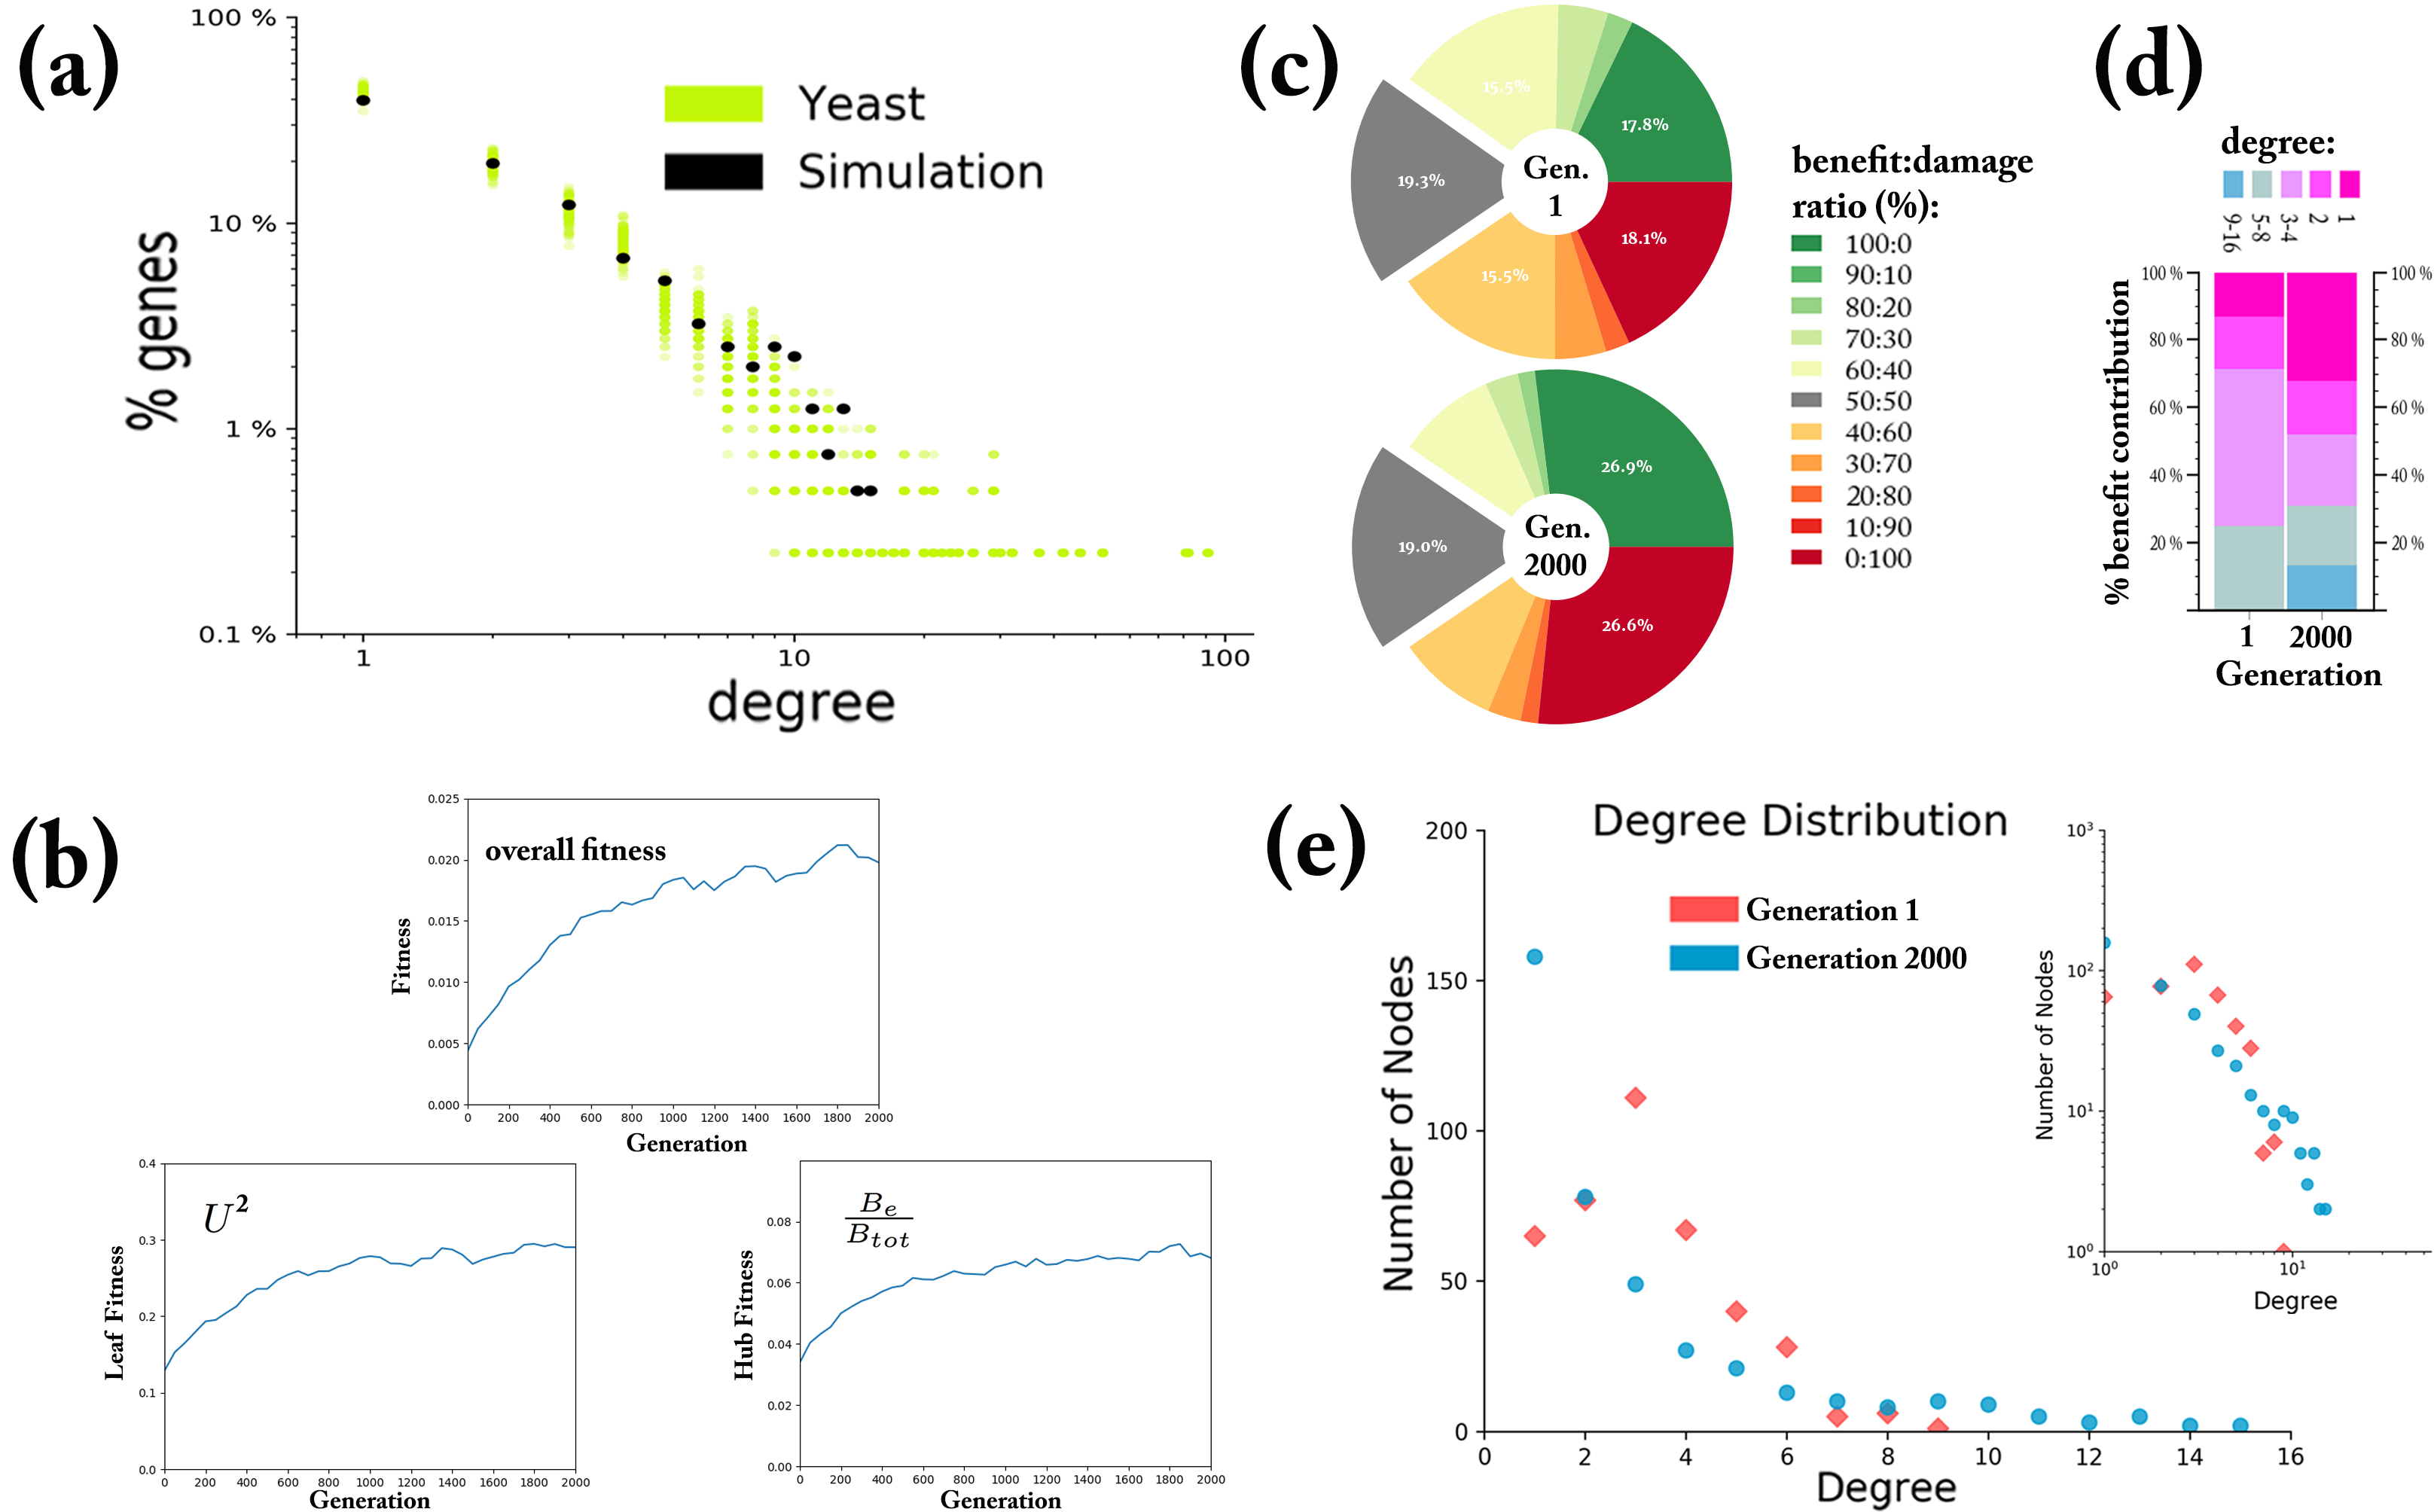
\includegraphics[scale=.65]{/adaptation/photoshop/processed_v5.png}
		\caption{Adaptation of a random seed network. 
					(a) starting from a network with the same  edge:node ratio as the Yeast network, but with edges randomly assigned to nodes, the mLmH property emerges after 2000 generations of random mutation (random edge re-assignment) and random selection according to instance size and effective total benefits.
					(b) Improvement in fitness over the generations.  The overall, $U$-only, and $\frac {B_e}{B_{tot}}$-only  fitness per generation depicted in top, bottom-left, bottom-right subplots respectively. 
					(c) The percentage of unambiguous genes in NEP increases over the course of simulated adaptation, resulting in easier instances with smaller effective instance sizes. Solid green (red) slices represent nodes with  zero damage and non-zero benefit (zero benefit and non-zero damage). Top pie: the initial random network at generation 1 includes on average 35.9\% unambiguous nodes; bottom pie: after 2000 generations, the network 
					has on average 53.5\% unambiguous nodes.
					(d) The percentage of benefits that nodes, grouped by degree range (legend, top), contribute to NEP solution before (generation 1 (left bar), random seed network) and after simulated adaptation (generation 2000, right bar). Larger nodes in adapted (generation 2000) network contribute a higher proportion of benefits due to the fact that the large number of damage-minimal leaves do not consume damage tolerance threshold thereby increasing the likelihood of (the more ambiguous and more tolerance-consuming) hubs to be in solution. The benefits in the solution for a random network  (generation 1) are predominantly contributed by medium degree nodes. After 2000 generations, a marked increase in the contribution by the majority leaves (degree 1 and 2 particularly) and by high degree hubs of degree $\geq$ 5 is observed. 
					(e) Initial random networks have exponential distributions. After simulated adaptation, mLmH topology emerges (more leaves and high-degree hubs in exchange for less medium-degree nodes);  inset: the same plot in log scale. 
		}
		\label{adap_fig}
\end{figure*}	

\begin{figure*}[t]
		\centering
		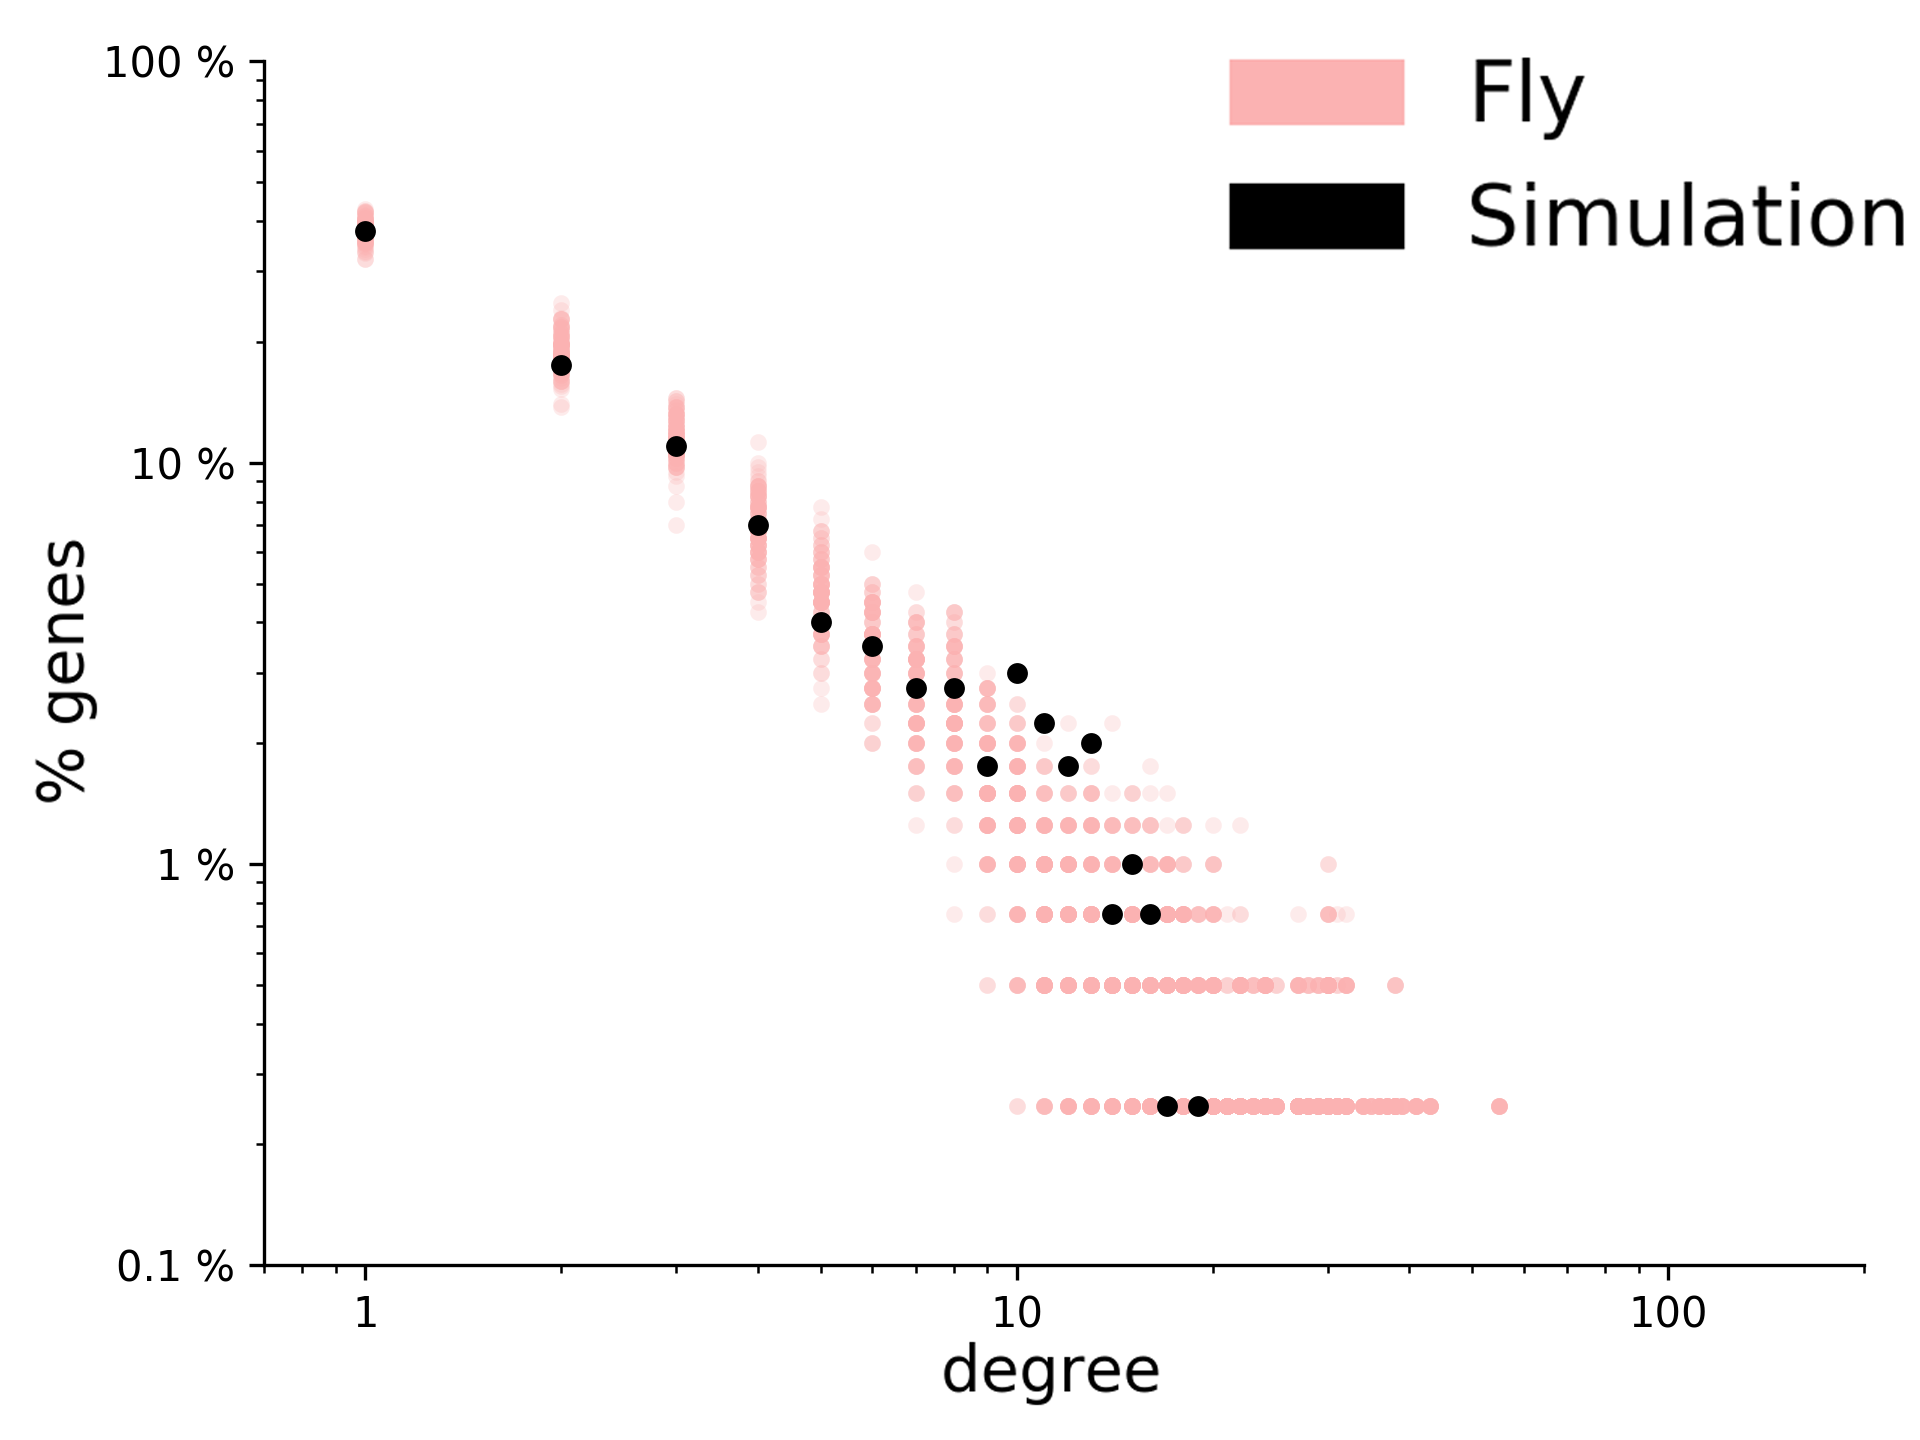
\includegraphics[scale=.36]{/adaptation_with_growth/faint_alpha/Evo_Fly.png}
		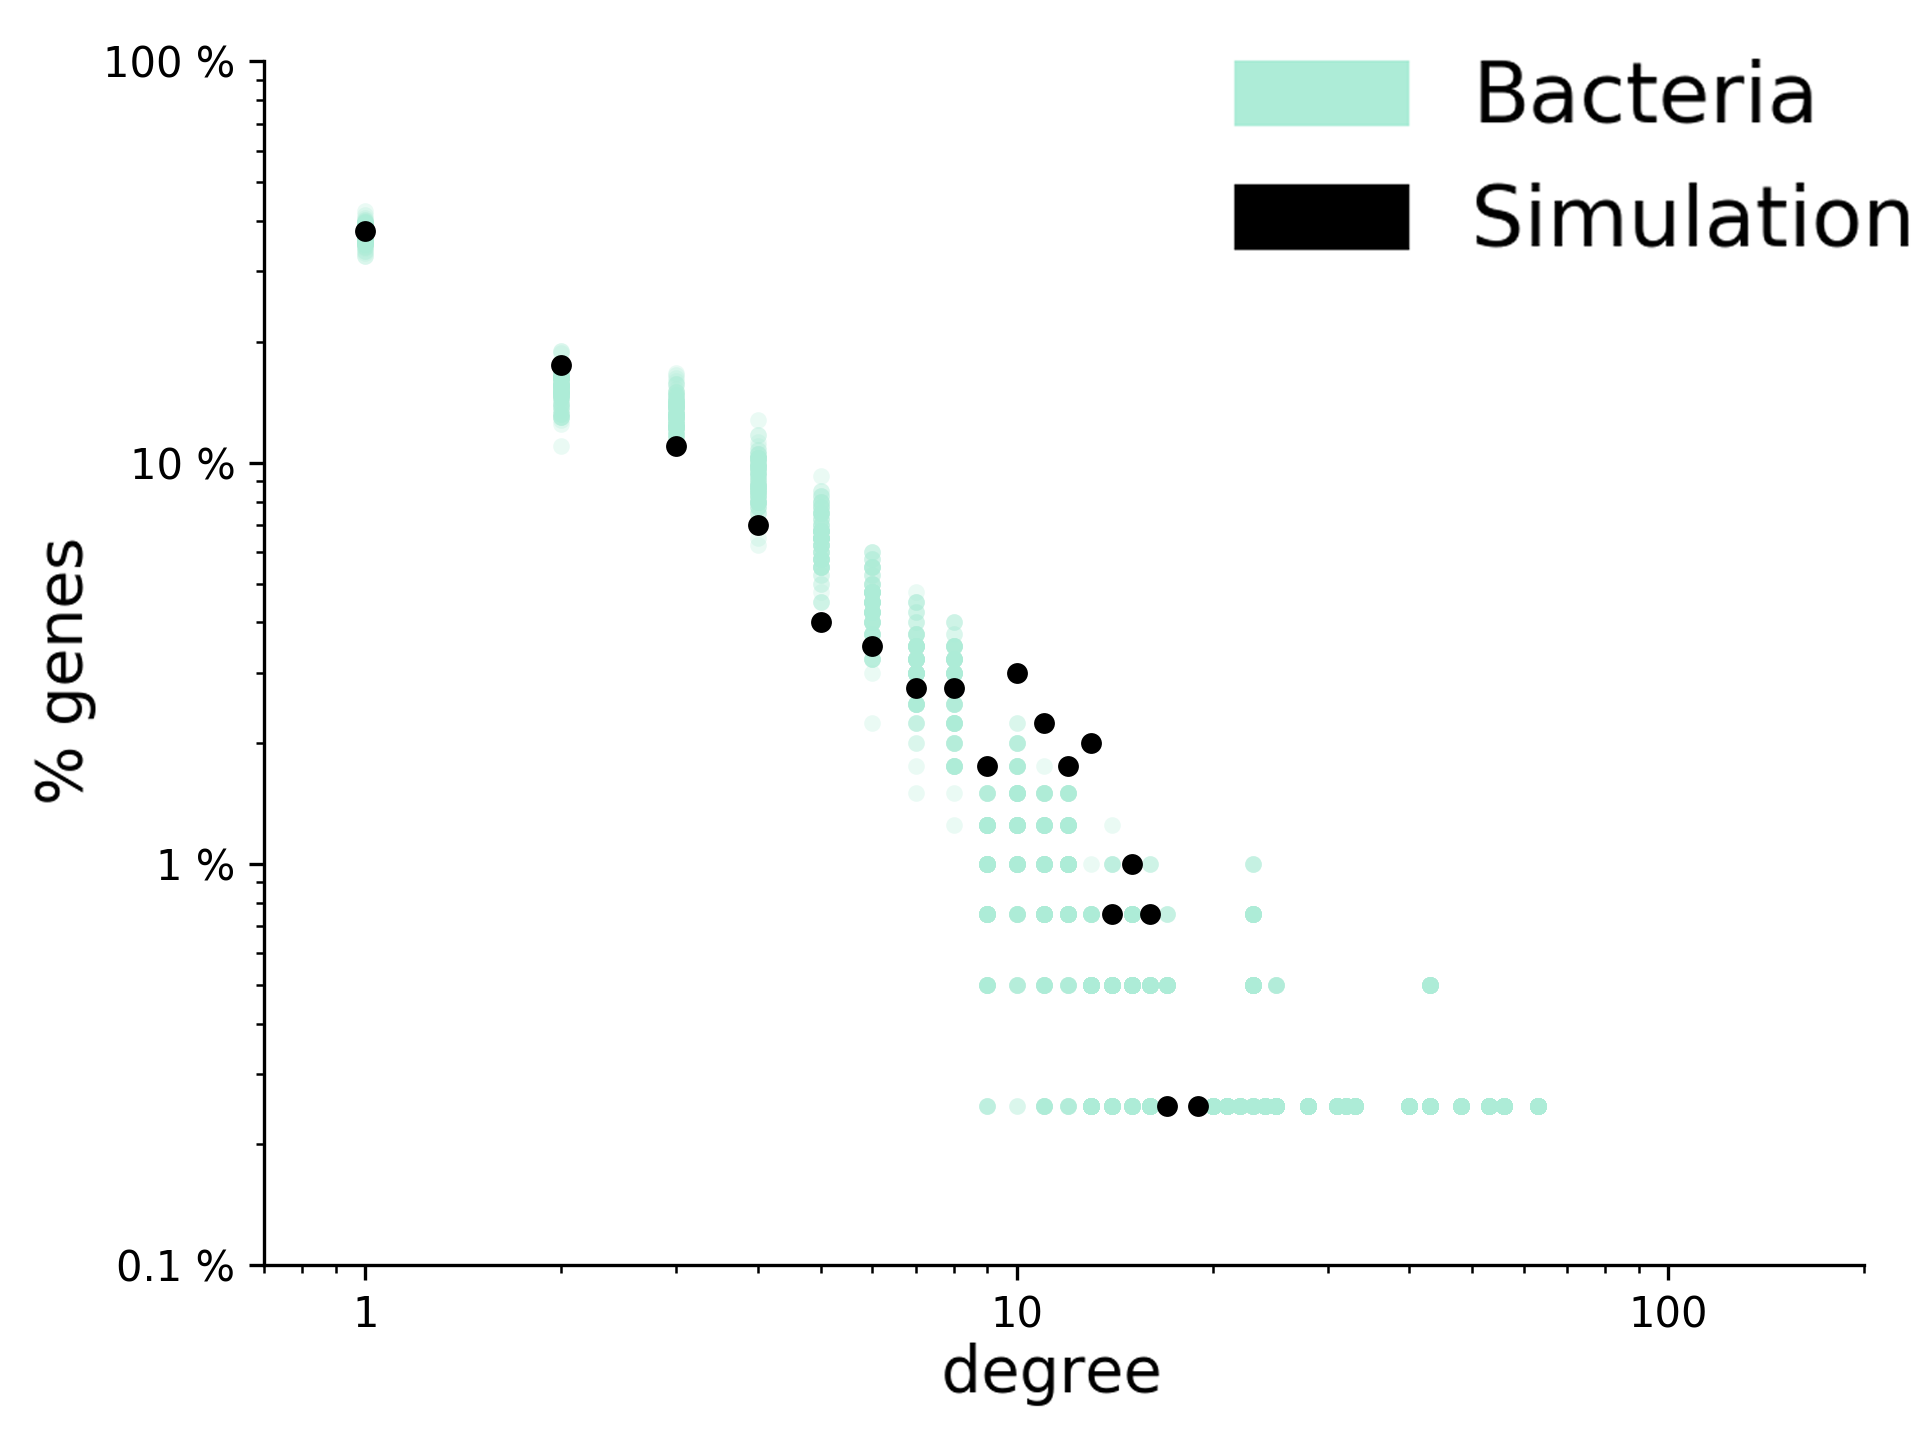
\includegraphics[scale=.36]{/adaptation_with_growth/faint_alpha/Evo_Bacteria.png}
		\includegraphics[scale=.36]{/adaptation_with_growth/faint_alpha/Evo_Humaniso.png}
		\\
		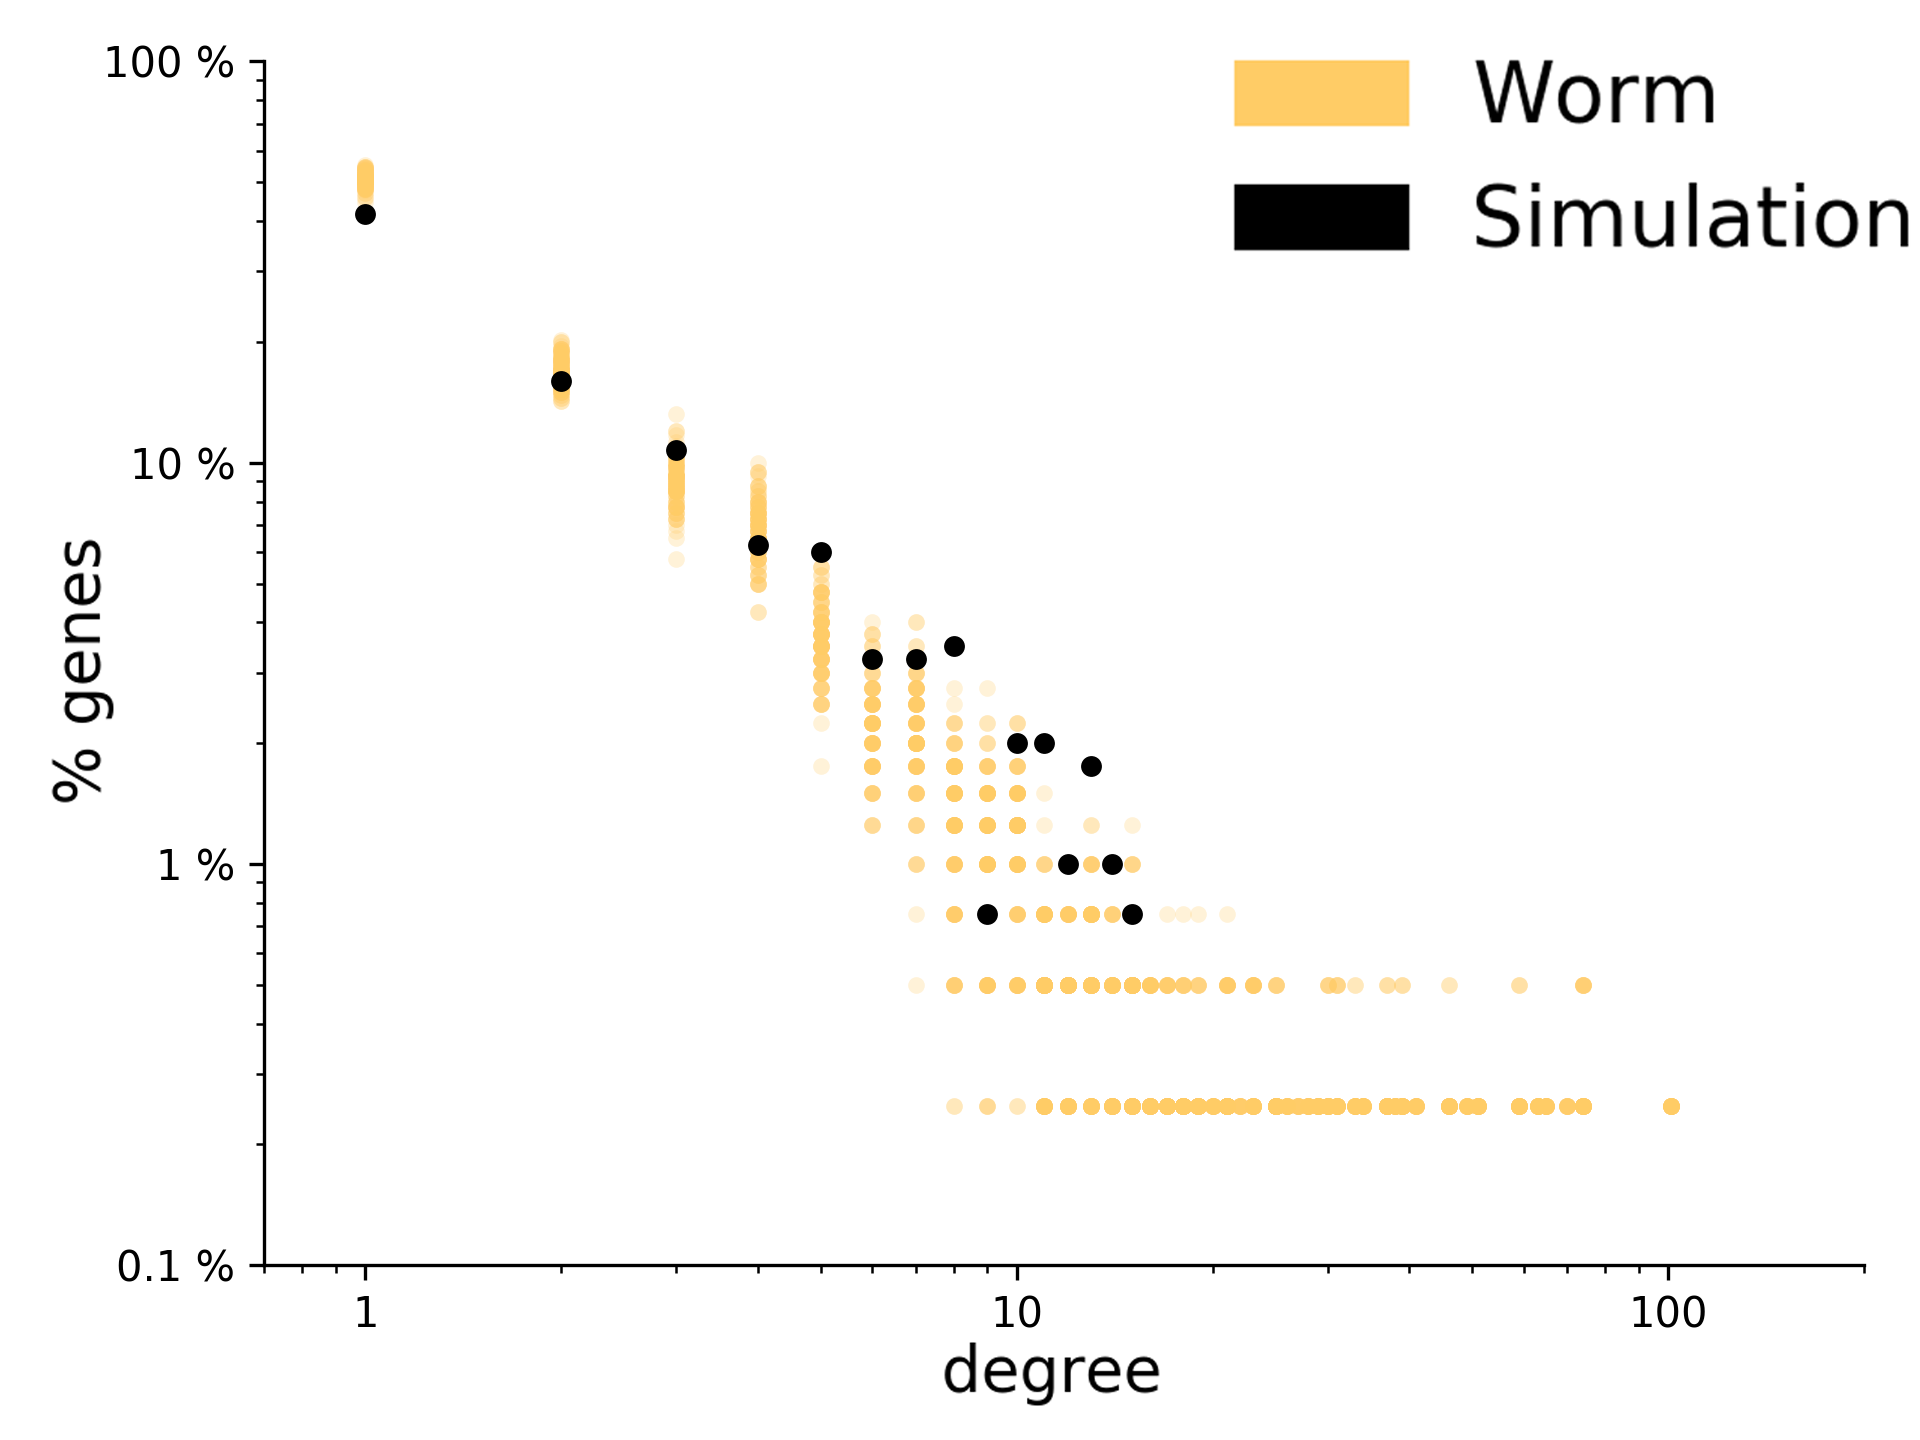
\includegraphics[scale=.36]{/adaptation_with_growth/faint_alpha/Evo_Worm.png}
		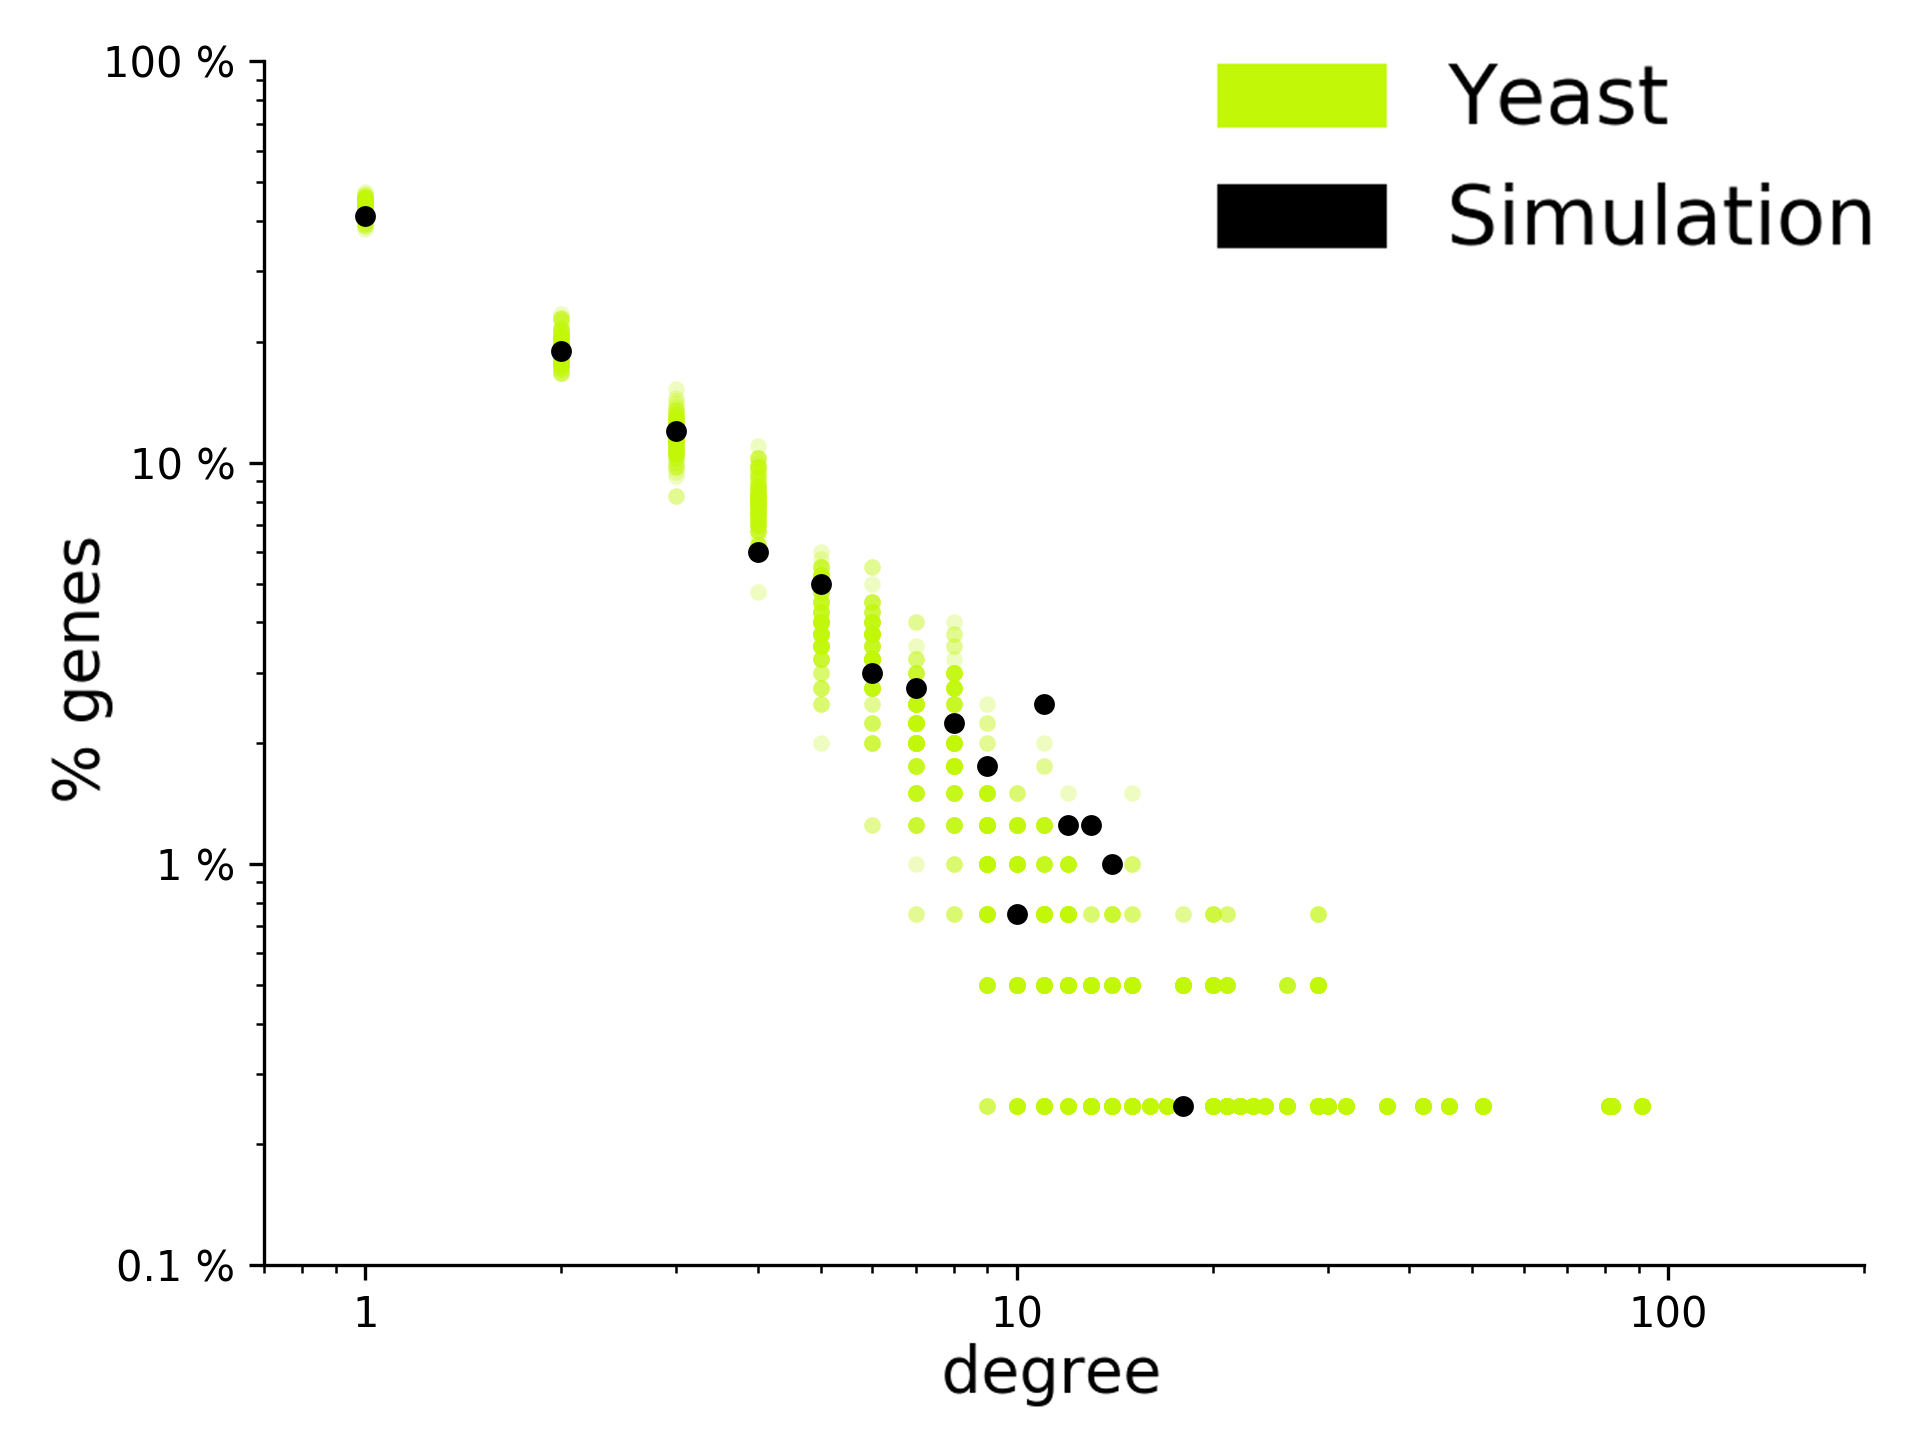
\includegraphics[scale=.36]{/adaptation_with_growth/faint_alpha/Evo_Yeast.png}
		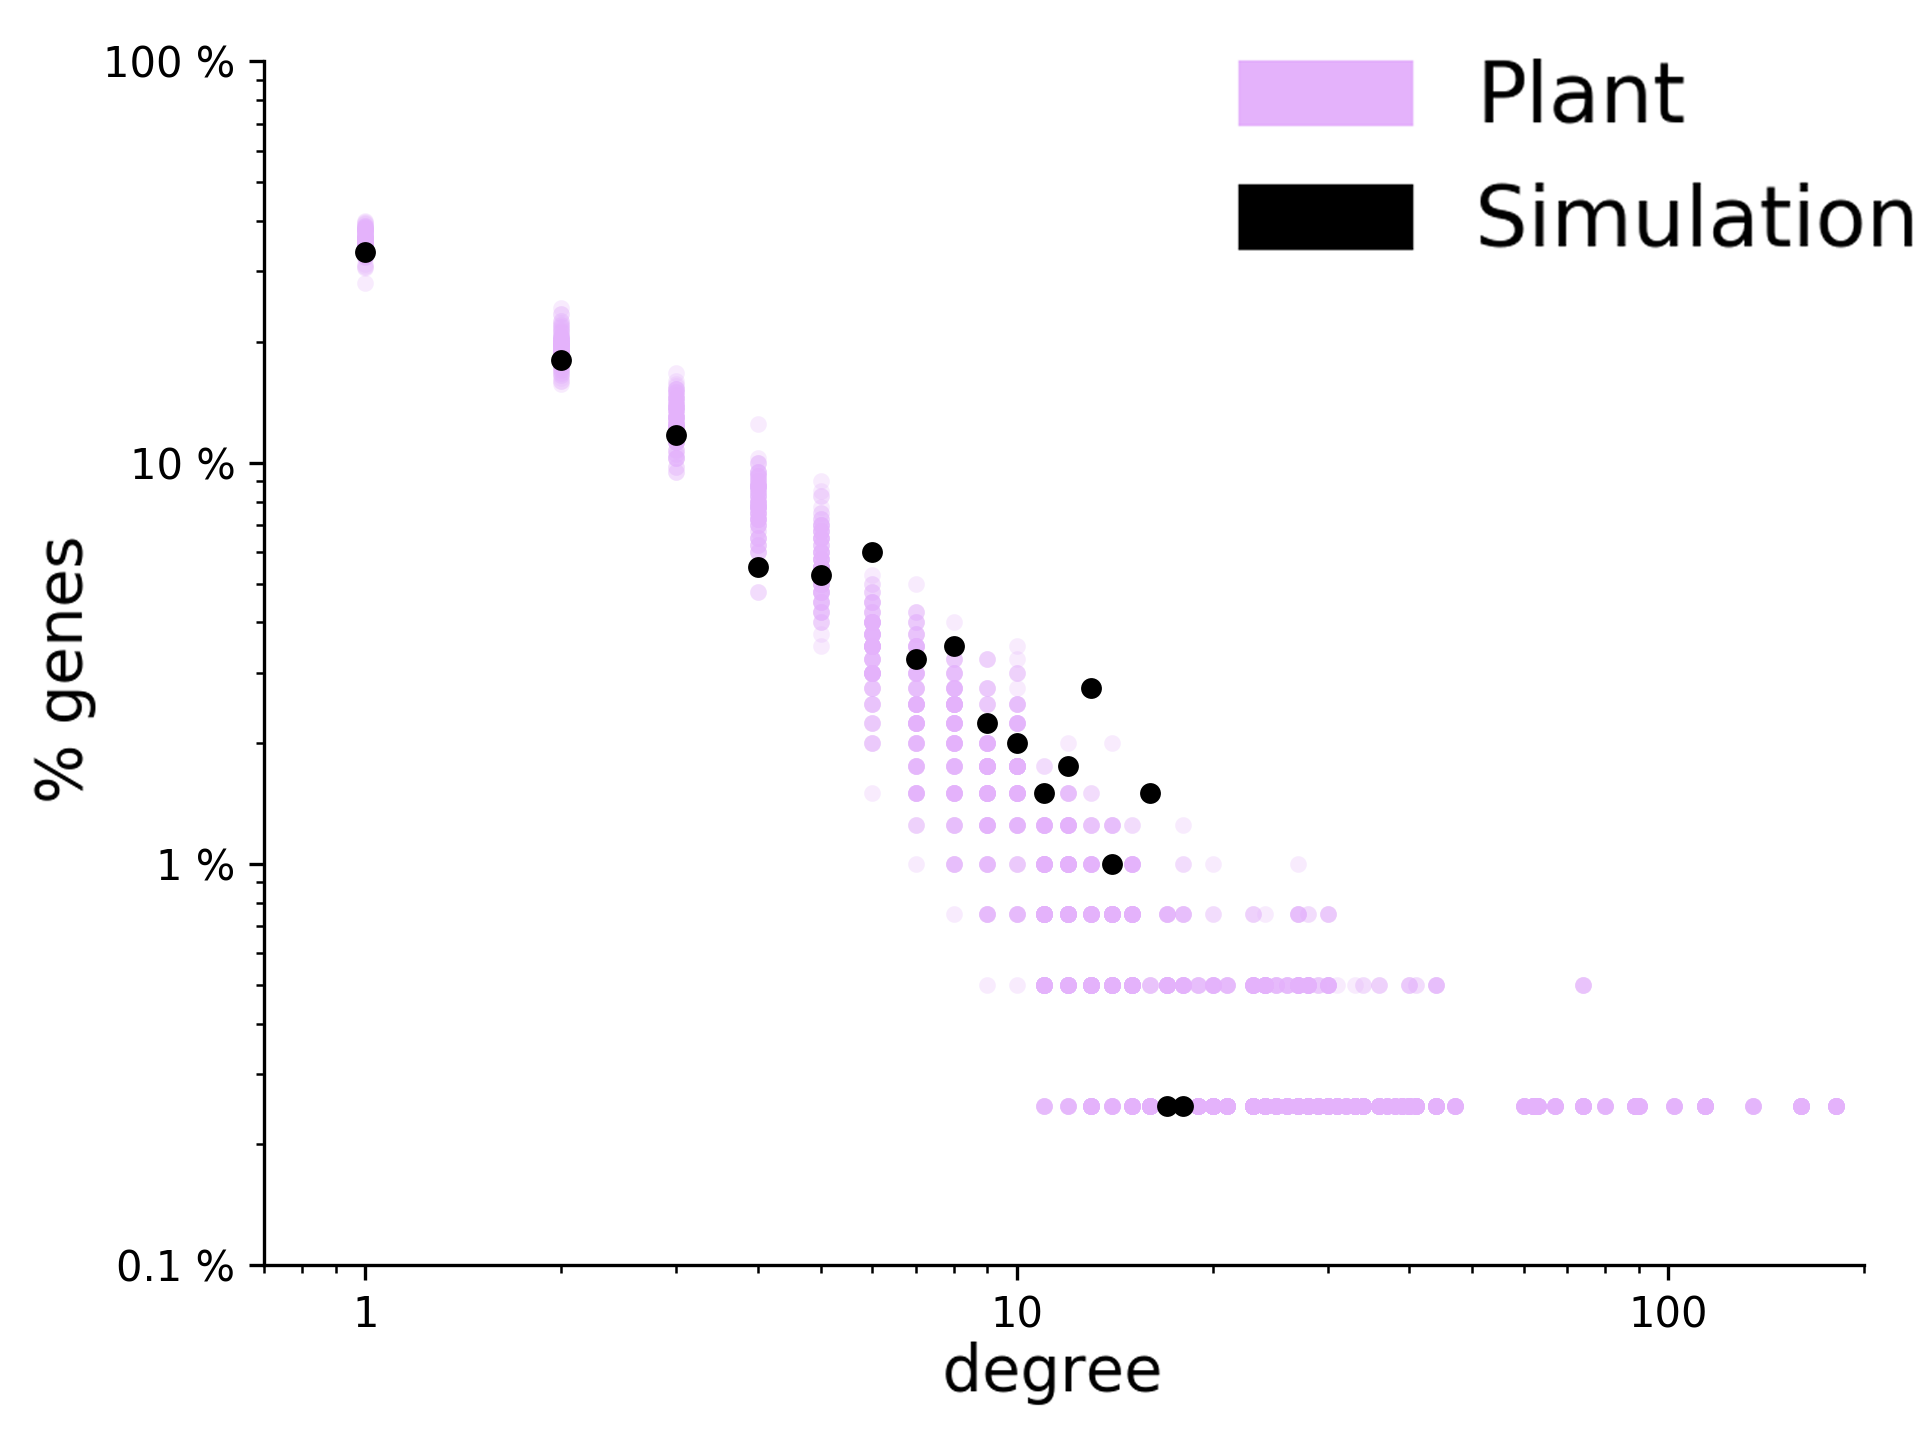
\includegraphics[scale=.36]{/adaptation_with_growth/faint_alpha/Evo_Plant.png}
		\caption{Adaptation with growth. Starting from a near empty network, evolution proceeds with mutations being random edge-reassignment  as 
		well as the addition of new nodes and edges. The size of the last network at algorithm termination is 400 nodes. The evolving networks 
		are not mutated with additional edges when their edge:node ratio exceeds that of the corresponding BN of the same edge:node ratio. 
		Shown here is the degree distribution of the fittest final network after 4000 generations of mutate-and-select (black dots), against the 
		degree distribution of 100 400-node randomly sampled subnetworks from each corresponding BN (colour dots). 
		In all cases, each evolved network's degree 
		distribution closely follows its corresponding BN of the same edge:node ratio.}
		\label{evol_figure} 
\end{figure*}	 
